
% ==================================================
%	Aufbau
% ==================================================

\section{Aufbau}

\subsection{Rauschspektrometer}
\label{sub:rauschspektrometer}

\begin{figure}[!htpb]
  \centering
  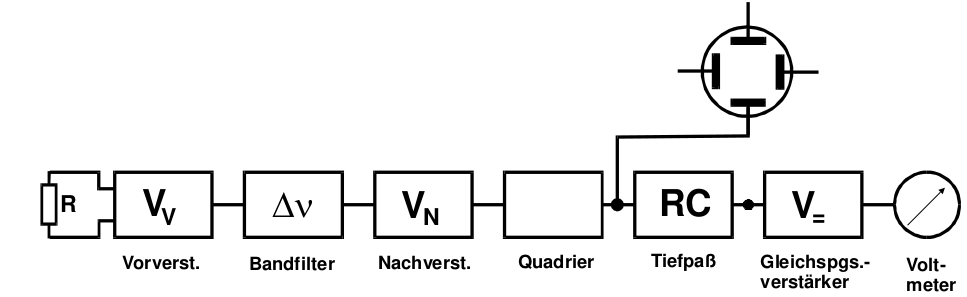
\includegraphics[scale=0.3]{bilder/spektrometer}
  \caption{Aufbau eines Rauschspektrometers.}
\label{fig:spektrometer}
\end{figure}

Der allgemeine Aufbau eines Rauschspektrometers ist in
Abbildung~\ref{fig:spektrometer} dargestellt.
Hierbei wird die an dem Widerstand abgegriffene Spannung mit einem
Verstärkungsfaktor $V_V$ verstärkt und anschließend durch einen Bandpassfilter
in einem Frequenzbereich $\Delta \nu$ gefiltert.
Das gefilterte Signal wird nun durch einen Faktor $V_N$ nachverstärkt,
quadriert und anschließend der Gleichspannungsanteil durch einen Tiefpass
herausgefiltert und nocheinmal mit einem Faktor $V_=$ verstärkt.
Das so bearbeitete Signal kann nun durch ein Voltmeter gemessen werden.
Dabei beträgt die gemessene Spannung
\begin{equation}
  U_a^2 = V_\text{ges} \Delta\nu 4 k_\text{B}TR \qquad \text{mit}\qquad
  V_\text{ges} = V_V\,V_N\,V_=~.
\end{equation}

\subsection{Korrelatorschaltung}
\label{sub:korrelatorschaltung}

Im Gegensatz zum Rauschspektrometer aus Abschnitt~\ref{sub:rauschspektrometer}
können durch zwei getrennt arbeitetende Verstärker deutlich geringere
Rauschspannungen gemessen werden, da diese unkorreliert sind.
Der Aufbau ist in Abbildung~\ref{fig:korrelator} dargestellt.
Hierbei der Aufbau aus Abschnitt~\ref{sub:rauschspektrometer} zweimal verwandt
und anstatt des Quadrierers werden die beiden Signale multipliziert bevor das
Signal am Tiefpass integriert wird.
Für die gemessene Spannung gilt näherungsweise
\begin{equation}
  U_{a,\text{korr}} = V_\text{ges}^2 \overline{U_R^2}~.
\end{equation}

\begin{figure}[htpb]
  \centering
  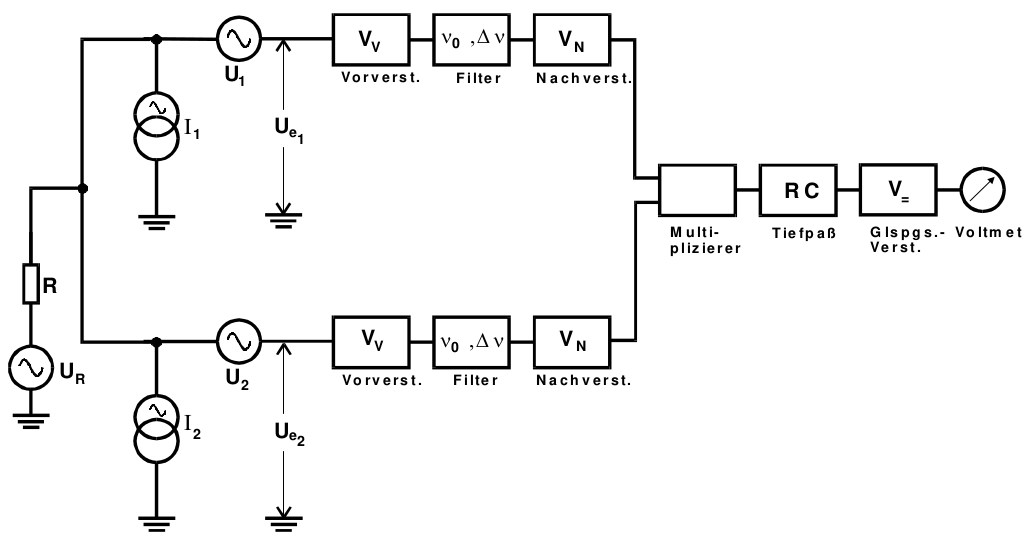
\includegraphics[scale=0.3]{bilder/korrelator.png}
  \caption{Aufbau der Korrelatorschaltung.}
\label{fig:korrelator}
\end{figure}

\subsection{Schrotrauschen}
\label{sub:schrotrauschen}

Zur Messung des Schrotrauschens einer Reinmetallkathode wird Röhre in der in
Abbildung~\ref{fig:spektrometer} dargestellt, wobei der Widerstand durch die
Diode ausgetauscht wird.
Die Funktionsweise ist analog zu Abschnitt~\ref{sub:rauschspektrometer}.

\subsection{Frequenzspektrum}
\label{sub:frequenzspektrum}

Zur Bestimmung der Frequenzspektren wird der Aufbau aus
Abbildung~\ref{fig:schrot} verwandt. Dieser Aufbau gleicht dem aus
Abbildung~\ref{fig:spektrometer} mit dem Unterschied, dass hier der
Bandpassfilter mit einem Selektivverstärker ausgetauscht ist.

\begin{figure}[htpb]
  \centering
  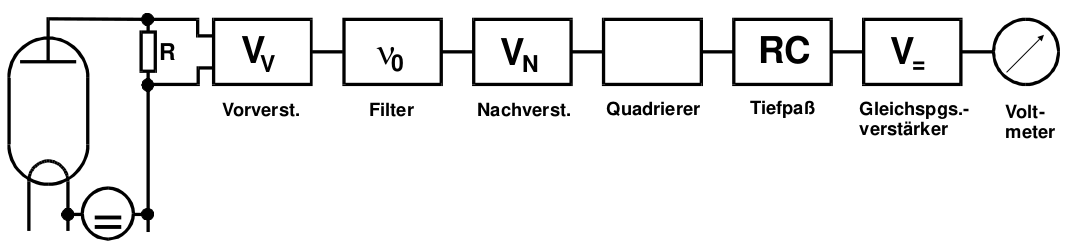
\includegraphics[scale=0.3]{bilder/schrot.png}
  \caption{Aufbau zur Messung des Rauschspektrums des Schroteffekts.}
\label{fig:schrot}
\end{figure}
